\documentclass[14pt,fleqn]{extarticle}
\RequirePackage{prepwell-eng}

\previewoff

\begin{document} 
\begin{skill}
\begin{narrow}
\textcolor{blue}{Angles of intersection}

Finding the intersection angles given the slopes of two lines; Condition for perpendicularity 
\end{narrow}

\reason 

In the figure below, two lines with slopes $m_1$ and $m_2$ intersect\newline 

Notice the triangle that has the $x-$axis as it's base. The three \underline{interior angles} of this triangle are 

\[\qquad \underbrace{\phi_2}_P,\underbrace{\pi-\phi_1}_Q\text{ and } \underbrace{B = \phi_1-\phi_2}_{\pi - (P+Q)} \]

\begin{center}
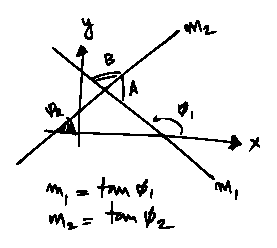
\includegraphics[scale=1.6]{figure.eps}
\end{center}

Both $A$ and $B$ are angles of intersection\newline 

However, \underline{by convention}, we report the angle of intersection as $\theta \leq 90^\circ$ \newline 

Which means $\theta = \tan^{-1}\left\vert \dfrac{m_1 - m_2}{1+m_1\cdot m_2}\right\vert$ \newline 

Also, if $\theta=90^\circ$, then $\tan\theta = \infty$. Or 
\[ 1 + m_1\cdot m_2 = 0 \implies \underbrace{m_1\cdot m_2 = -1}_{\text{Condition for orthogonality}} \]

\end{skill} 
\end{document}
